\documentclass[12pt]{standalone}

\usepackage[utf8]{inputenc}
\usepackage[T1]{fontenc}
\usepackage[svgnames]{xcolor}

\usepackage{tikz}
\usepackage{tikz-qtree}
\usetikzlibrary{fit,backgrounds}

\title{The Extremity-Conditionally-on-Nonmidpoint (ECN) Model}

\author{Hansjörg Plieninger}

\begin{document}

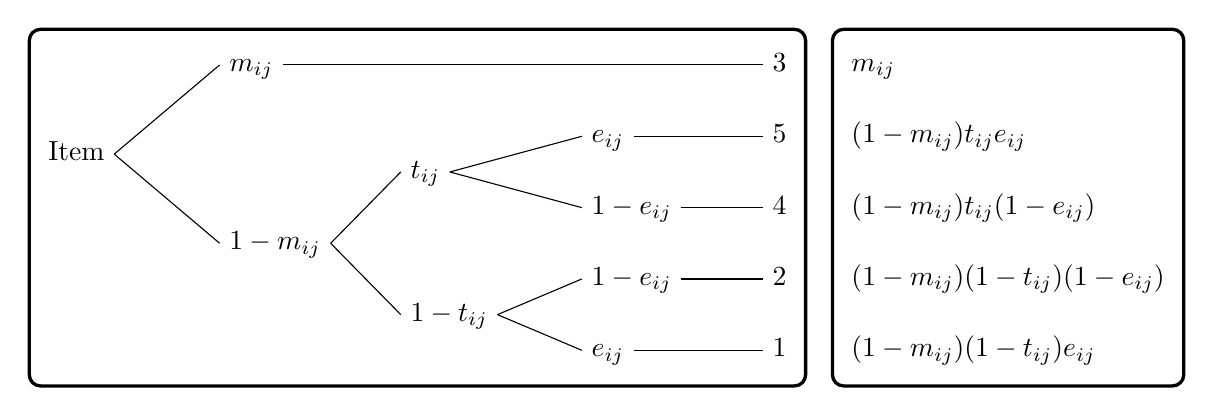
\begin{tikzpicture}
\tikzset{grow'=right,level distance=23mm, sibling distance=2.5mm}
\tikzset{level 5/.style={level distance=10mm}}
\tikzset{execute at begin node=\strut}
\tikzset{every tree node/.style={anchor=base west, align=left, font = \normalsize}}
\tikzset{ri style/.style={font=\scriptsize, auto=right, midway}}
\tikzset{le style/.style={font=\scriptsize, auto=left,  midway}}
%\tikzset{frontier/.style={distance from root=.8\linewidth}}

\Tree [.\node(I){Item}; [.\node(M1){$m_{ij}$}; 
[.{} [.{} [.\node(C3){3}; \edge[draw=none]; \node(E3){$m_{ij}$};] ] ] ]
[.\node(M2){$1-m_{ij}$};
[.\node(T1){$t_{ij}$}; 
[.\node(T1E1){$e_{ij}$};  [.\node(C5){5}; \edge[draw=none]; \node(E5){$(1-m_{ij})t_{ij}e_{ij}$};]]
[.\node(T1E2){$1-e_{ij}$};  [.\node(C4){4}; \edge[draw=none]; \node(E4){$(1-m_{ij}) t_{ij} (1-e_{ij})$}; ]]]
[.\node(T2){$1-t_{ij}$}; 
[.\node(T2E2){$1-e_{ij}$};  [.\node(C2){2}; \edge[draw=none]; \node(E2){$(1-m_{ij}) (1-t_{ij}) (1-e_{ij})$}; ]]
[.\node(T2E1){$e_{ij}$};  [.\node(C1){1}; \edge[draw=none]; \node(E1){$(1-m_{ij})(1-t_{ij})e_{ij}$};]] ]  ]
]
\draw[-] (M1)--(C3);
\begin{scope}[on background layer]
\node[draw, rounded corners, fill=none, color=Black, very thick, fit=(E3)(E2)(E1)]{};
\node[draw, rounded corners, fill=none, color=Black, very thick, fit=(I)(C3)(C1)]{};
\end{scope} 
\end{tikzpicture}

\end{document}
